\documentclass{scrartcl}

\usepackage{amssymb}
\usepackage{amsmath}
\usepackage{tikz}
\usetikzlibrary{calc,intersections,through,backgrounds,patterns}
\usetikzlibrary{decorations.text, decorations.markings, fit, arrows, arrows.meta}

\begin{document}
	
	%\begin{figure}
	%	\centering
	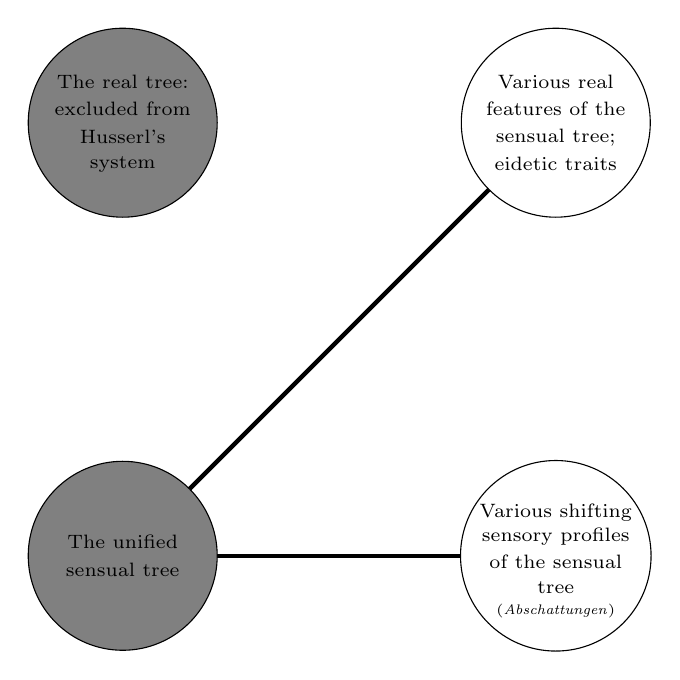
\begin{tikzpicture}
	%lines
	\draw[ultra thick] (0,0)--(5.5,5.5);
	\draw[ultra thick] (0,0)--(5.5,0);
	
	%circles
	\filldraw[draw,fill=gray] (0,0) circle (1.2cm);
	\filldraw[draw,fill=gray] (0,5.5) circle (1.2cm);
	\filldraw[draw,fill=white] (5.5,5.5) circle (1.2cm);
	\filldraw[draw,fill=white] (5.5,0) circle (1.21cm);
	
	%inner labels
	\node at (0,6.025) {{\scriptsize The real tree:}};
	\node at (0,5.675) {{\scriptsize excluded from}};
	\node at (0,5.325) {{\scriptsize Husserl's}};
	\node at (0,4.975) {{\scriptsize system}};
	%
	\node at (5.5,6.025) {{\scriptsize Various real}};
	\node at (5.5,5.675) {{\scriptsize features of the}};
	\node at (5.5,5.315) {{\scriptsize sensual tree;}};
	\node at (5.5,4.975) {{\scriptsize eidetic traits}};
	%
	\node at (0,0.175)  {{\scriptsize The unified}}; 
	\node at (0,-0.175) {{\scriptsize sensual tree}}; 
	%
	\node at (5.5,0.55)  {{\scriptsize Various shifting}}; 
	\node at (5.5,0.24)  {{\scriptsize sensory profiles}}; 
	\node at (5.5,-0.07) {{\scriptsize of the sensual}}; 
	\node at (5.5,-0.4)  {{\scriptsize tree}}; 
	\node at (5.5,-0.7)  {{\tiny (\textit{Abschattungen})}};
	
	%\draw[help lines] (0,0) grid (6,6);
	\end{tikzpicture}
	%	\caption{Two Tensions in Sensual Objects (Husserl)}		%p. 33
	%\end{figure}
	
	
	\vspace{3cm}
	
	
	%\begin{figure}
	%	\centering
	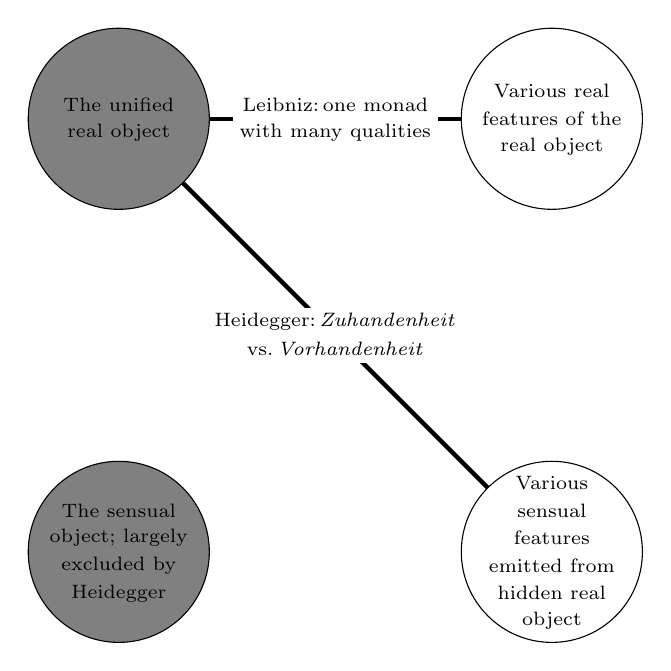
\begin{tikzpicture}
	%lines
	\draw[ultra thick] (0,5.5)--(5.5,5.5);
	\draw[ultra thick] (0,5.5)--(5.5,0);
		\fill[white] (1.45,5.2) rectangle (4.05,5.8);	%manual fill - Leibniz
		\fill[white] (1.1,2.4) rectangle (4.4,3.1);		%manual fill - Heidegger
		
	%circles
	\filldraw[draw,fill=gray] (0,0) circle (1.15cm);
	\filldraw[draw,fill=gray] (0,5.5) circle (1.15cm);
	\filldraw[draw,fill=white] (5.5,5.5) circle (1.15cm);
	\filldraw[draw,fill=white] (5.5,0) circle (1.15cm);
	
	%inner labels
	\node at (0,5.675) {{\scriptsize The unified}};
	\node at (0,5.325) {{\scriptsize real object}};
	%
	\node at (5.5,5.85) {{\scriptsize Various real}};
	\node at (5.5,5.5)  {{\scriptsize features of the}};
	\node at (5.5,5.15) {{\scriptsize real object}};
	%
	\node at (0,0.525)  {{\scriptsize The sensual}}; 
	\node at (0,0.175)  {{\scriptsize object; largely}}; 
	\node at (0,-0.175) {{\scriptsize excluded by}}; 
	\node at (0,-0.525) {{\scriptsize Heidegger}};
	%
	\node at (5.5,0.875)  {{\scriptsize Various}}; 
	\node at (5.5,0.525)  {{\scriptsize sensual}}; 
	\node at (5.5,0.175)  {{\scriptsize features}}; 
	\node at (5.5,-0.175) {{\scriptsize emitted from}}; 
	\node at (5.5,-0.525) {{\scriptsize hidden real}};
	\node at (5.5,-0.875) {{\scriptsize object}};
	
	%outer labels
	\node at (2.75,5.675) {{\scriptsize Leibniz:$\,$one monad}};
	\node at (2.75,5.325) {{\scriptsize with many qualities}};
	%
	\node at (2.75,2.925) {{\scriptsize Heidegger:$\,$\textit{Zuhandenheit}}};
	\node at (2.75,2.575) {{\scriptsize vs.$\,$\textit{Vorhandenheit}}};
	
	%\draw[help lines] (0,0) grid (6,6);
	\end{tikzpicture}
	%	\caption{Two Tensions in Real Objects (Heidegger and Leibniz)}	%p. 48
	%\end{figure}
	
	
	\vspace{3cm}
	
	
	%\begin{figure}
	%	\centering
	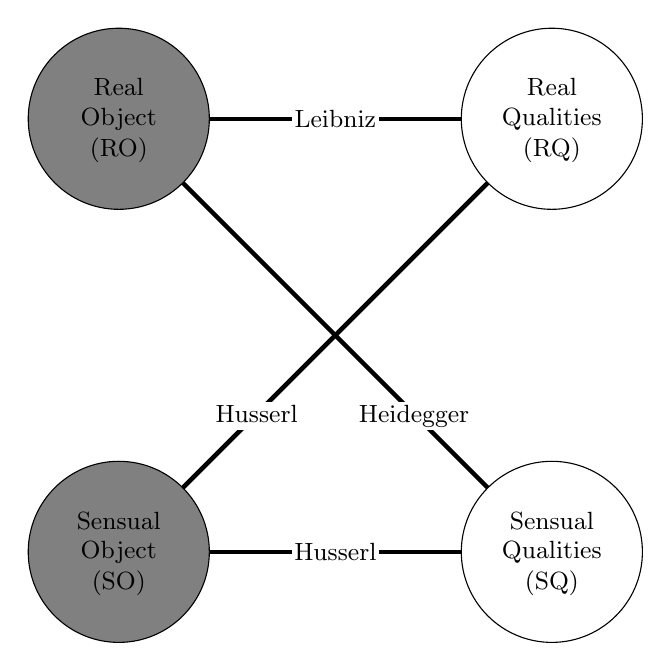
\begin{tikzpicture}
	%lines
	\draw[ultra thick] (0,5.5)--(5.5,5.5);
	\draw[ultra thick] (0,5.5)--(5.5,0);
	\draw[ultra thick] (5.5,5.5)--(0,0);
	\draw[ultra thick] (0,0)--(5.5,0);
	\fill[white] (2.2,5.3) rectangle (3.3,5.65);	%manual fill - Leibniz
	\fill[white] (1.2,1.55) rectangle (2.3,1.9);	%manual fill - Husserl (left)
	\fill[white] (3,1.55) rectangle (4.5,1.9);		%manual fill - Heidegger
	\fill[white] (2.2,0.2) rectangle (3.3,-0.2);	%manual fill - Husserl  (bottom)
	
	%circles
	\filldraw[draw,fill=gray] (0,0) circle (1.15cm);
	\filldraw[draw,fill=gray] (0,5.5) circle (1.15cm);
	\filldraw[draw,fill=white] (5.5,5.5) circle (1.15cm);
	\filldraw[draw,fill=white] (5.5,0) circle (1.15cm);
	
	%inner labels
	\node at (0,5.9) {{\small Real}};
	\node at (0,5.5) {{\small Object}};
	\node at (0,5.1) {{\small (RO)}};
	%
	\node at (5.5,5.9) {{\small Real}};
	\node at (5.5,5.5) {{\small Qualities}};
	\node at (5.5,5.1) {{\small (RQ)}};
	%
	\node at (0,0.4)  {{\small Sensual}}; 
	\node at (0,0.0)  {{\small Object}}; 
	\node at (0,-0.4) {{\small (SO)}};
	%
	\node at (5.5,0.4)  {{\small Sensual}}; 
	\node at (5.5,0) 	{{\small Qualities}}; 
	\node at (5.5,-0.4) {{\small (SQ)}}; 
	
	%outer labels
	\node at (2.75,5.5)  {{\small Leibniz}};
	\node at (1.75,1.75) {{\small Husserl}};
	\node at (3.75,1.72) {{\small Heidegger}};
	\node at (2.75,0) 	 {{\small Husserl}};
	
	%\draw[help lines] (0,0) grid (6,6);
	\end{tikzpicture}
	%	\caption{The Fourfold Structure Emerges}	%p. 50
	%\end{figure}
	
	
	\vspace{3cm}
	
	
	\hspace{-1.25cm}		%this is just to center the diagram; remove if used elsewhere
	%\begin{figure}
	%	\centering
	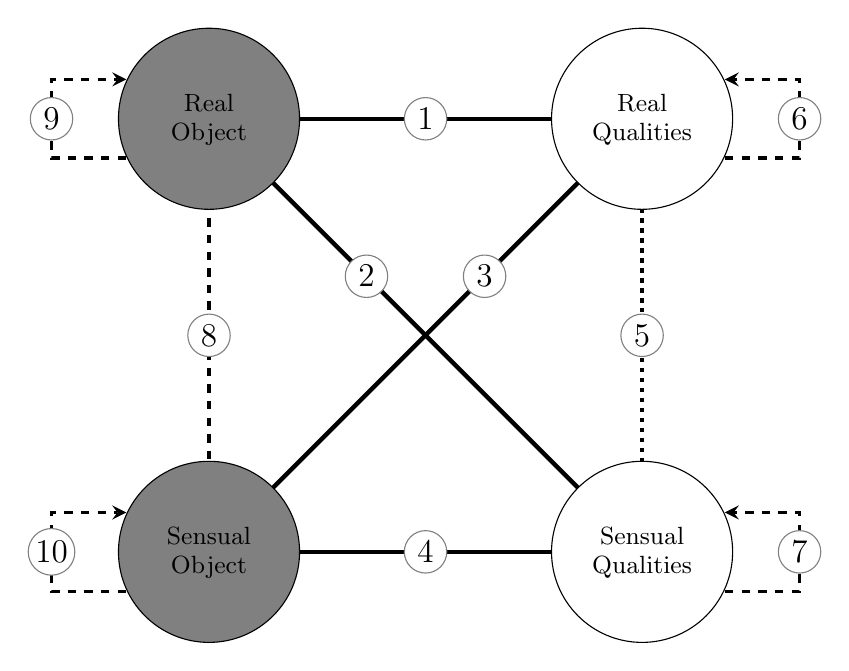
\begin{tikzpicture}
	%lines
	\draw[ultra thick] (0,5.5)--(5.5,5.5);
	\draw[ultra thick] (0,5.5)--(5.5,0);
	\draw[ultra thick] (5.5,5.5)--(0,0);
	\draw[ultra thick] (0,0)--(5.5,0);
	\draw[ultra thick,dashed] (0,5.5)--(0,0);
	\draw[ultra thick,dotted] (5.5,5.5)--(5.5,0);
	
	%boxes
	\draw[->,>=stealth,very thick,dashed] (0,5)--(-2,5)--(-2,6)--(-1.05,6);
	\draw[->,>=stealth,very thick,dashed] (0,-0.5)--(-2,-0.5)--(-2,0.5)--(-1.05,0.5);
	\draw[->,>=stealth,very thick,dashed] (5.5,5)--(7.5,5)--(7.5,6)--(6.55,6);
	\draw[->,>=stealth,very thick,dashed] (5.5,-0.5)--(7.5,-0.5)--(7.5,0.5)--(6.55,0.5);
	
	%circles
	\filldraw[draw,fill=gray] (0,0) circle (1.15cm);
	\filldraw[draw,fill=gray] (0,5.5) circle (1.15cm);
	\filldraw[draw,fill=white] (5.5,5.5) circle (1.15cm);
	\filldraw[draw,fill=white] (5.5,0) circle (1.15cm);
	
	%inner labels
	\node at (0,5.7) {{\small Real}};
	\node at (0,5.3) {{\small Object}};
	%
	\node at (5.5,5.7) {{\small Real}};
	\node at (5.5,5.3) {{\small Qualities}};
	%
	\node at (0,0.2)  {{\small Sensual}}; 
	\node at (0,-.2)  {{\small Object}}; 
	%
	\node at (5.5,0.2)  {{\small Sensual}}; 
	\node at (5.5,-.2) 	{{\small Qualities}};
	
	%circled numbers
	\filldraw (2.75,5.5)node[circle,inner sep=2pt,draw=gray,fill=white] {{\large 1}};
	\filldraw (2,3.5)   node[circle,inner sep=2pt,draw=gray,fill=white] {{\large 2}};
	\filldraw (3.5,3.5) node[circle,inner sep=2pt,draw=gray,fill=white] {{\large 3}};
	\filldraw (2.75,0)  node[circle,inner sep=2pt,draw=gray,fill=white] {{\large 4}};
	\filldraw (5.5,2.75)node[circle,inner sep=2pt,draw=gray,fill=white] {{\large 5}};
	\filldraw (7.5,5.5) node[circle,inner sep=2pt,draw=gray,fill=white] {{\large 6}};
	\filldraw (7.5,0)   node[circle,inner sep=2pt,draw=gray,fill=white] {{\large 7}};
	\filldraw (0,2.75)  node[circle,inner sep=2pt,draw=gray,fill=white] {{\large 8}};
	\filldraw (-2,5.5)  node[circle,inner sep=2pt,draw=gray,fill=white] {{\large 9}};
	\filldraw (-2,0)    node[circle,inner sep=1pt,draw=gray,fill=white] {{\large 10}};
	
	%\draw[help lines] (0,0) grid (6,6);
	\end{tikzpicture}
	%	\caption{The Ten Possible Links}	%p. 78
	%\end{figure}
	
	
	\vspace{3cm}
	
	
	%\begin{figure}
	%	\centering
	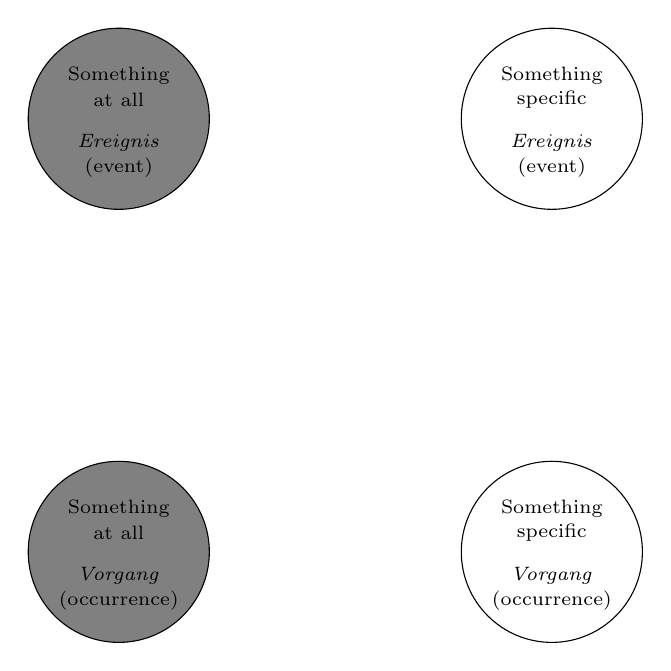
\begin{tikzpicture}
	%circles
	\filldraw[draw,fill=gray] (0,0) circle (1.15cm);
	\filldraw[draw,fill=gray] (0,5.5) circle (1.15cm);
	\filldraw[draw,fill=white] (5.5,5.5) circle (1.15cm);
	\filldraw[draw,fill=white] (5.5,0) circle (1.15cm);
	
	%inner labels
	\node at (0,6.05) {{\scriptsize Something}};
	\node at (0,5.74) {{\scriptsize at all}};
	\node at (0,5.2)  {{\scriptsize \textit{Ereignis}}};
	\node at (0,4.88) {{\scriptsize (event)}};
	%
	\node at (5.5,6.05) {{\scriptsize Something}};
	\node at (5.5,5.74) {{\scriptsize specific}};
	\node at (5.5,5.2)  {{\scriptsize \textit{Ereignis}}};
	\node at (5.5,4.88) {{\scriptsize (event)}};
	%
	\node at (0,0.55)  {{\scriptsize Something}}; 
	\node at (0,0.24)  {{\scriptsize at all}}; 
	\node at (0,-0.3)  {{\scriptsize \textit{Vorgang}}}; 
	\node at (0,-0.62) {{\scriptsize (occurrence)}}; 
	%
	\node at (5.5,0.55)  {{\scriptsize Something}}; 
	\node at (5.5,0.24)  {{\scriptsize specific}}; 
	\node at (5.5,-0.3)  {{\scriptsize \textit{Vorgang}}}; 
	\node at (5.5,-0.62) {{\scriptsize (occurrence)}};
	\end{tikzpicture}
	%	\caption{Heidegger's Early Fourfold (1919)}		%p. 89
	%\end{figure}
	
	
	\vspace{3cm}
	
	
	%\begin{figure}
	%	\centering
	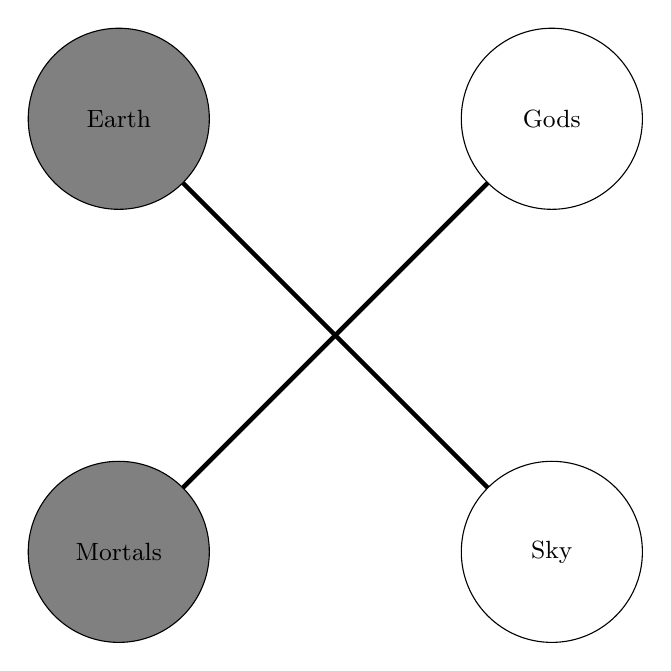
\begin{tikzpicture}
	%lines
	\draw[ultra thick] (0,5.5)--(5.5,0);
	\draw[ultra thick] (0,0)--(5.5,5.5);
	
	%circles
	\filldraw[draw,fill=gray] (0,0) circle (1.15cm);
	\filldraw[draw,fill=gray] (0,5.5) circle (1.15cm);
	\filldraw[draw,fill=white] (5.5,5.5) circle (1.15cm);
	\filldraw[draw,fill=white] (5.5,0) circle (1.15cm);
	
	%inner labels
	\node at (0,5.5)   {{\small Earth}};
	\node at (5.5,5.5) {{\small Gods}};
	\node at (0,0.0)   {{\small Mortals}}; 
	\node at (5.5,0)   {{\small Sky}}; 
	\end{tikzpicture}
	%	\caption{Heidegger's Late Fourfold (1949)}	%p. 89
	%\end{figure}
	
	
	\vspace{3cm}
	
	
	%\begin{figure}
	%	\centering
	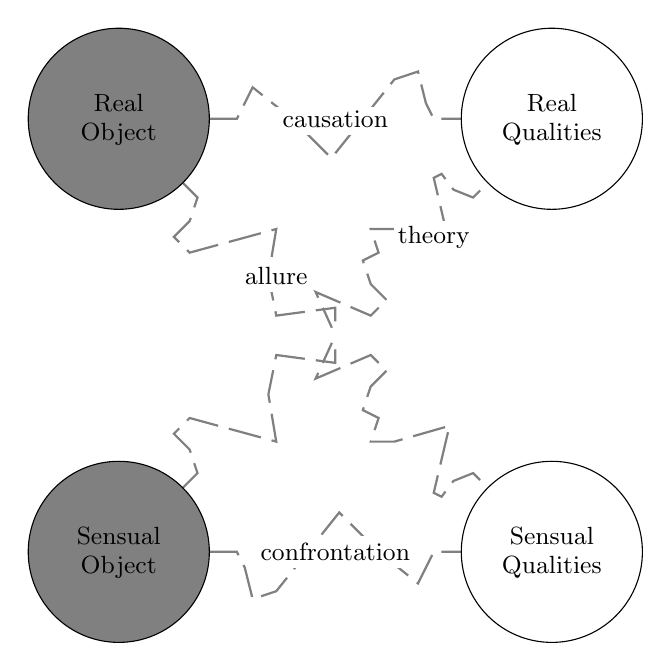
\begin{tikzpicture}
	%lines
	\draw[thick,gray,dash pattern=on 12pt off 4pt] (0,5.5)--(1.5,5.5)--(1.7,5.9)--(2.2,5.5)--(2.7,5)--(3.5,6)--(3.8,6.1)--(3.9,5.7)--(4,5.5)--(5.5,5.5);
	%
	\draw[thick,gray,dash pattern=on 12pt off 4pt] (0,5.5)--(1,4.5)--(0.9,4.2)--(0.7,4)--(0.9,3.8)--(2,4.1)--(1.9,3.5)--(2,3)--(2.75,3.1)--(2.75,2.75)--(2.5,2.2)--(3.2,2.5)--(3.4,2.3)--(3.2,2.1)--(3.1,1.8)--(3.3,1.7)--(3.2,1.4)--(3.5,1.4)--(4.2,1.6)--(4,0.75)--(4.1,0.7)--(4.25,0.9)--(4.5,1)--(5.5,0);		%diagonal (#21)
	%
	\draw[thick,gray,dash pattern=on 12pt off 4pt] (0,0)--(1,1)--(0.9,1.3)--(0.7,1.5)--(0.9,1.7)--(2,1.4)--(1.9,2)--(2,2.5)--(2.75,2.4)--(2.75,2.75)--(2.5,3.3)--(3.2,3)--(3.4,3.2)--(3.2,3.4)--(3.1,3.7)--(3.3,3.8)--(3.2,4.1)--(3.5,4.1)--(4.2,3.9)--(4,4.75)--(4.1,4.8)--(4.25,4.6)--(4.5,4.5)--(5.5,5.5);		%off-diagonal
	%
	%(0,0)--(1,1)--(1.25,0.9)--(1.4,0.7)--(1.5,0.75)--(1.3,1.6)--(2,1.4)--(2.3,1.4)--(2.2,1.7)--(2.4,1.8)--(2.3,2.1)--(2.1,2.3)--(2.3,2.5)--(3,2.3)--(2.75,2.75)--(2.75,3.1)--(3.5,3)--(3.6,3.5)--(3.5,4.1)--(4.6,3.8)--(4.8,4)--(4.6,4.2)--(4.5,4.5)--(5.5,5.5);
	%
	\fill[white] (2.75,2.75) circle (3pt); 	%hack to cover ugly crossover in middle
	%
	\draw[thick,gray,dash pattern=on 12pt off 4pt] (0,0)--(1.5,0)--(1.6,-0.2)--(1.7,-0.6)--(2,-0.5)--(2.8,0.5)--(3.3,0)--(3.8,-0.4)--(4,0)--(5.5,0);
	%
	\fill[white] (2,5.3) rectangle (3.5,5.65);		%manual fill - causation
	\fill[white] (1.6,3.3) rectangle (2.4,3.65);	%manual fill - allure
	\fill[white] (3.5,3.9) rectangle (4.5,4.2);		%manual fill - theory
	\fill[white] (1.7,0.2) rectangle (3.8,-0.2);	%manual fill - confrontation
	
	%the diagonal and off-diagonal lines are mirror images of one another: backwards & upside-down
	%If we have one line, reverse its values. Then for both axes, calculate the differences between steps.
	%starting at (0,0), add the differences to the x-axis & subtract them from the y-axis, up to (5.5,5.5)
	
	%circles
	\filldraw[draw,fill=gray] (0,0) circle (1.15cm);
	\filldraw[draw,fill=gray] (0,5.5) circle (1.15cm);
	\filldraw[draw,fill=white] (5.5,5.5) circle (1.15cm);
	\filldraw[draw,fill=white] (5.5,0) circle (1.15cm);
	
	%inner labels
	\node at (0,5.7) {{\small Real}};
	\node at (0,5.3) {{\small Object}};
	%
	\node at (5.5,5.7) {{\small Real}};
	\node at (5.5,5.3) {{\small Qualities}};
	%
	\node at (0,0.2) {{\small Sensual}}; 
	\node at (0,-.2) {{\small Object}}; 
	%
	\node at (5.5,0.2) {{\small Sensual}}; 
	\node at (5.5,-.2) {{\small Qualities}};
	
	%outer labels
	\node at (2.75,5.5){{\small causation}}; 
	\node at (2,3.5)   {{\small allure}}; 
	\node at (4,4) 	   {{\small theory}}; 
	\node at (2.75,0)  {{\small confrontation}}; 
	
	%\draw[help lines] (0,0) grid (6,6);
	\end{tikzpicture}
	%	\caption{Broken Links}	%p. 107
	%\end{figure}
	
	
	\vspace{3cm}
	
	
	%\begin{figure}
	%	\centering
	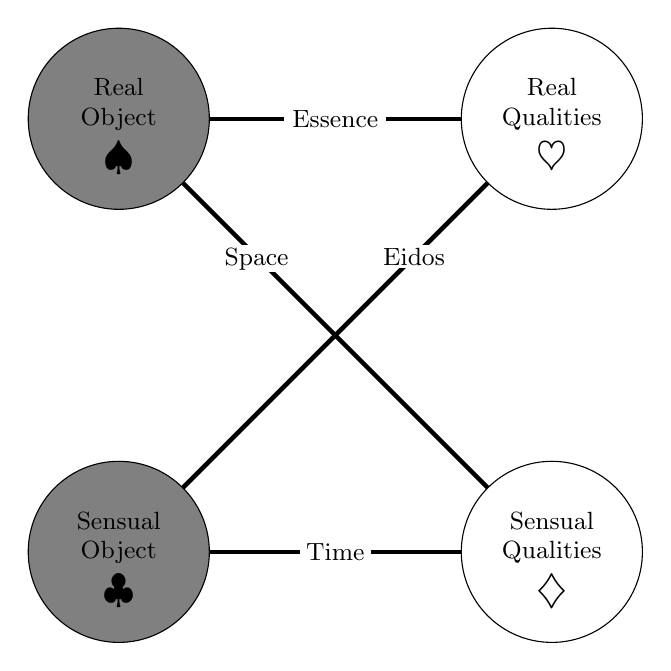
\begin{tikzpicture}
	%lines
	\draw[ultra thick] (0,5.5)--(5.5,5.5);
	\draw[ultra thick] (0,5.5)--(5.5,0);
	\draw[ultra thick] (5.5,5.5)--(0,0);
	\draw[ultra thick] (0,0)--(5.5,0);
	\fill[white] (2.1,5.3) rectangle (3.4,5.65);	%manual fill - Essence
	\fill[white] (1.3,3.55) rectangle (2.2,3.9);	%manual fill - Space
	\fill[white] (3.3,3.6) rectangle (4.2,3.9);		%manual fill - Eidos
	\fill[white] (2.3,0.2) rectangle (3.2,-0.2);	%manual fill - Time
	
	%circles
	\filldraw[draw,fill=gray] (0,0) circle (1.15cm);
	\filldraw[draw,fill=gray] (0,5.5) circle (1.15cm);
	\filldraw[draw,fill=white] (5.5,5.5) circle (1.15cm);
	\filldraw[draw,fill=white] (5.5,0) circle (1.15cm);
	
	%inner labels
	\node at (0,5.9) {{\small Real}};
	\node at (0,5.5) {{\small Object}};
	\node at (0,5)   {{\Large $\spadesuit$}};
	%
	\node at (5.5,5.9) {{\small Real}};
	\node at (5.5,5.5) {{\small Qualities}};
	\node at (5.5,5)   {{\Large $\heartsuit$}};
	%
	\node at (0,0.4)  {{\small Sensual}}; 
	\node at (0,0.0)  {{\small Object}}; 
	\node at (0,-0.5) {{\Large $\clubsuit$}};
	%
	\node at (5.5,0.4)  {{\small Sensual}}; 
	\node at (5.5,0) 	{{\small Qualities}}; 
	\node at (5.5,-0.5) {{\Large $\diamondsuit$}}; 
	
	%outer labels
	\node at (2.75,5.5)  {{\small Essence}};
	\node at (1.75,3.72) {{\small Space}};
	\node at (3.75,3.75) {{\small Eidos}};
	\node at (2.75,0) 	 {{\small Time}};
	
	%\draw[help lines] (0,0) grid (6,6);
	\end{tikzpicture}
	%	\caption{The Four Tensions}	%p. 114
	%\end{figure}
	
	
	\vspace{3cm}
	
	
	%\begin{figure}
	%	\centering
	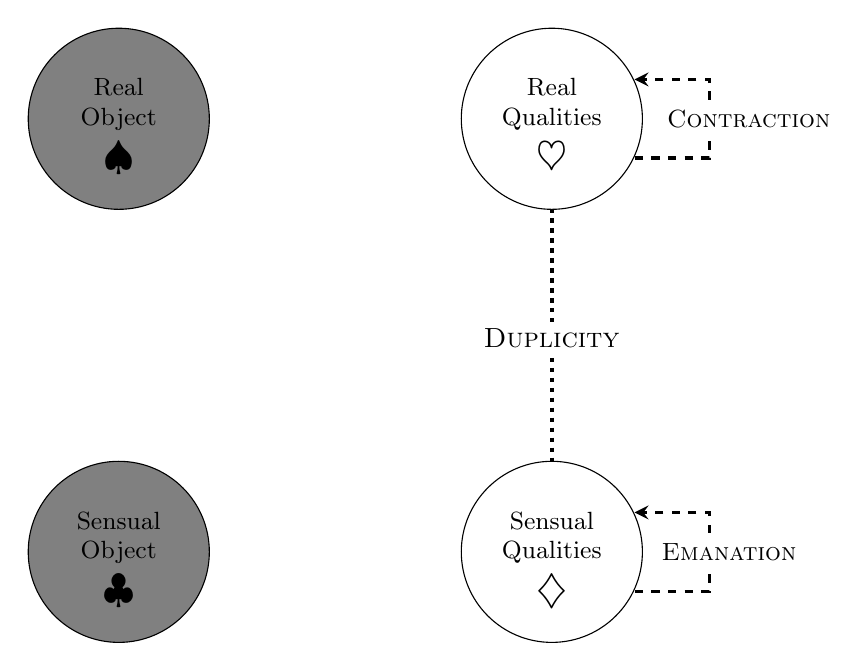
\begin{tikzpicture}
	%lines
	\draw[ultra thick,dotted] (5.5,5.5)--(5.5,0);
	\draw[->,>=stealth,very thick,dashed] (5.5,5)--(7.5,5)--(7.5,6)--(6.55,6);				%top box
	\draw[->,>=stealth,very thick,dashed] (5.5,-0.5)--(7.5,-0.5)--(7.5,0.5)--(6.55,0.5);	%bottom box
	\fill[white] (6.8,5.3) rectangle (9.15,5.65);	%manual fill - Contraction
	\fill[white] (4.6,2.5) rectangle (6.4,2.9);		%manual fill - Duplicity
	\fill[white] (6.8,-0.2) rectangle (8.75,0.15);	%manual fill - Emanation
	
	%circles
	\filldraw[draw,fill=gray] (0,0) circle (1.15cm);
	\filldraw[draw,fill=gray] (0,5.5) circle (1.15cm);
	\filldraw[draw,fill=white] (5.5,5.5) circle (1.15cm);
	\filldraw[draw,fill=white] (5.5,0) circle (1.15cm);
	
	%inner labels
	\node at (0,5.9) {{\small Real}};
	\node at (0,5.5) {{\small Object}};
	\node at (0,5)   {{\Large $\spadesuit$}};
	%
	\node at (5.5,5.9) {{\small Real}};
	\node at (5.5,5.5) {{\small Qualities}};
	\node at (5.5,5)   {{\Large $\heartsuit$}};
	%
	\node at (0,0.4)  {{\small Sensual}}; 
	\node at (0,0.0)  {{\small Object}}; 
	\node at (0,-0.5) {{\Large $\clubsuit$}};
	%
	\node at (5.5,0.4)  {{\small Sensual}}; 
	\node at (5.5,0) 	{{\small Qualities}}; 
	\node at (5.5,-0.5) {{\Large $\diamondsuit$}}; 
	
	%outer labels
	\node at (8,5.5)	{{\small \textsc{Contraction}}};
	\node at (5.5,2.72) {{\textsc{Duplicity}}};
	\node at (7.75,0)	{{\small \textsc{Emanation}}};
	
	%\draw[help lines] (0,0) grid (9,6);
	\end{tikzpicture}
	%	\caption{The Three Radiations}	%p. 114
	%\end{figure}
	
	
	\vspace{3cm}
	
	
	\hspace{-2.5cm}
	%\begin{figure}
	%	\centering
	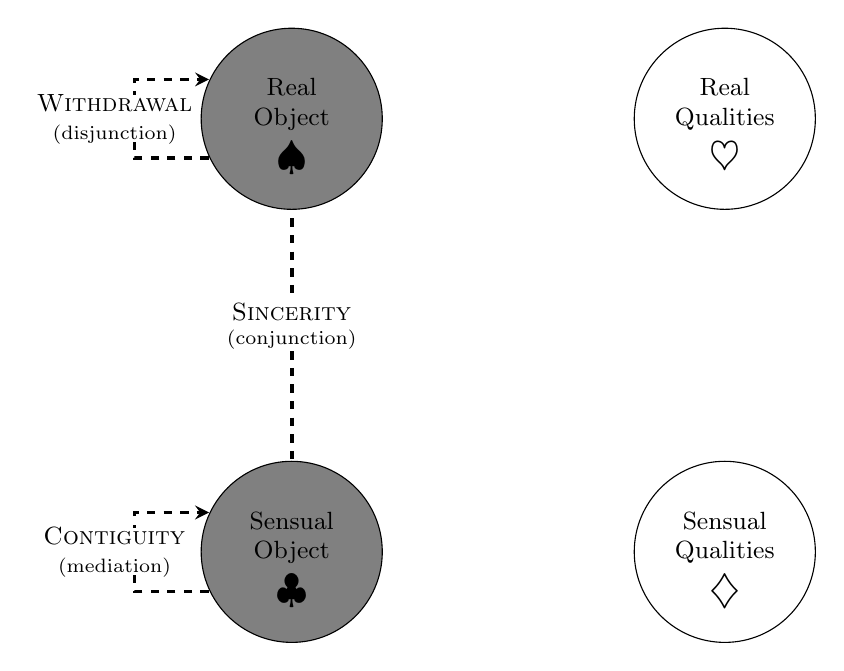
\begin{tikzpicture}
	%lines
	\draw[ultra thick,dashed] (0,5.5)--(0,0);
	\draw[->,>=stealth,very thick,dashed] (0,5)--(-2,5)--(-2,6)--(-1.05,6);				%top box
	\draw[->,>=stealth,very thick,dashed] (0,-0.5)--(-2,-0.5)--(-2,0.5)--(-1.05,0.5);	%bottom box
	\fill[white] (-3.3,5.2) rectangle (-1.4,5.8);	%manual fill - Withdrawal
	\fill[white] (-1,2.6) rectangle (1,3.2);		%manual fill - Sincerity
	\fill[white] (-3.3,-0.3) rectangle (-1.5,0.3);	%manual fill - Contiguity
	
	%circles
	\filldraw[draw,fill=gray] (0,0) circle (1.15cm);
	\filldraw[draw,fill=gray] (0,5.5) circle (1.15cm);
	\filldraw[draw,fill=white] (5.5,5.5) circle (1.15cm);
	\filldraw[draw,fill=white] (5.5,0) circle (1.15cm);
	
	%inner labels
	\node at (0,5.9) {{\small Real}};
	\node at (0,5.5) {{\small Object}};
	\node at (0,5)   {{\Large $\spadesuit$}};
	%
	\node at (5.5,5.9) {{\small Real}};
	\node at (5.5,5.5) {{\small Qualities}};
	\node at (5.5,5)   {{\Large $\heartsuit$}};
	%
	\node at (0,0.4)  {{\small Sensual}}; 
	\node at (0,0.0)  {{\small Object}}; 
	\node at (0,-0.5) {{\Large $\clubsuit$}};
	%
	\node at (5.5,0.4)  {{\small Sensual}}; 
	\node at (5.5,0) 	{{\small Qualities}}; 
	\node at (5.5,-0.5) {{\Large $\diamondsuit$}}; 
	
	%outer labels
	\node at (-2.25,5.7) {{\small \textsc{Withdrawal}}};
	\node at (-2.25,5.3) {{\scriptsize (disjunction)}};
	\node at (0,3.05) 	 {{\small \textsc{Sincerity}}};
	\node at (0,2.7)	 {{\scriptsize (conjunction)}};
	\node at (-2.25,0.2) {{\small \textsc{Contiguity}}};
	\node at (-2.25,-.2) {{\scriptsize (mediation)}};
	
	%\draw[help lines] (-3,0) grid (6,6);
	\end{tikzpicture}
	%	\caption{The Three Junctions}	%p. 115
	%\end{figure}
\end{document}